\documentclass[11pt,a4paper]{article}

\usepackage[utf8]{inputenc}
\usepackage[T1]{fontenc}
\usepackage{lmodern}
\usepackage[margin=2.5cm,headheight=14.5pt]{geometry}
\usepackage{graphicx}
\usepackage{booktabs}
\usepackage{amsmath,amssymb}
\usepackage{fancyhdr}
\usepackage{hyperref}
\usepackage{listings}
\usepackage{xcolor}
\usepackage{float}
\usepackage{pgfplots}
\usepackage{subcaption}
\usepackage{microtype}
\pgfplotsset{compat=1.18}

\hypersetup{
    colorlinks=true,
    linkcolor=black,
    citecolor=black,
    filecolor=black,
    urlcolor=blue,
    pdftitle={Laboratory Work No. 1: Concurrency in Practice},
    pdfauthor={Strunga Daniel-Ioan}
}

% Marker for values that still have to be measured / filled in.
\newcommand{\tbd}[1][TBD]{\textcolor{red}{\textbf{[#1]}}}

% Running header and footer
\pagestyle{fancy}
\fancyhf{}
\lhead{Laboratory Work No. 1 --- Network Programming}
\rhead{Strunga Daniel-Ioan}
\cfoot{\thepage}
\renewcommand{\headrulewidth}{0.4pt}
\renewcommand{\footrulewidth}{0pt}

% Code listing configuration
\definecolor{codebg}{RGB}{250, 250, 250}
\definecolor{commentgreen}{RGB}{46, 139, 87}
\lstset{
    backgroundcolor=\color{codebg},
    basicstyle=\ttfamily\footnotesize,
    breaklines=true,
    frame=single,
    rulecolor=\color{lightgray},
    commentstyle=\color{commentgreen}\itshape,
    keywordstyle=\bfseries\color{blue},
    showstringspaces=false,
    tabsize=2
}

\begin{document}

% =========================================================================
% TITLE PAGE
% =========================================================================
\begin{titlepage}
\begin{center}
    \vspace*{0.5cm}
    {\Large \textbf{TECHNICAL UNIVERSITY OF MOLDOVA}}\\[0.2cm]
    {\large Faculty of Computers, Informatics and Microelectronics}\\[0.15cm]
    {\large Department of Software Engineering and Automatics}\\[1.5cm]

    
\includegraphics[width=4.5cm]{figures/utm_logo.png}\\[1.8cm]

    {\LARGE \textbf{LABORATORY WORK NO. 1}}\\[0.4cm]
    {\Large \textbf{Concurrency in Practice: Multithreading,}}\\[0.2cm]
    {\Large \textbf{Shared State, and I/O Performance Analysis}}\\[0.5cm]
    {\large Course: Network Programming}\\[3.5cm]

    \begin{minipage}{0.48\textwidth}
        \textbf{Author:}\\
        Daniel-Ioan \textsc{Strunga}\\
        Student of group: FAF-242
    \end{minipage}
    \hfill
    \begin{minipage}{0.48\textwidth}
        \begin{flushright}
            \textbf{Verified by:}\\
            Lecturer / Supervisor\\
            Ernest \textsc{Bîtca}
        \end{flushright}
    \end{minipage}

    \vfill
    {\large Chișinău --- 2026}
\end{center}
\end{titlepage}

% =========================================================================
% TABLE OF CONTENTS
% =========================================================================
\newpage
\pagenumbering{arabic}
\setcounter{page}{1}

\tableofcontents
\newpage

% =========================================================================
% SECTION 1: INTRODUCTION AND OBJECTIVES
% =========================================================================
\section{Introduction and Laboratory Objectives}

Concurrent and parallel execution is fundamental to network programming and high-performance distributed systems. Understanding how modern operating system threads interact with multi-core processor architectures, memory hierarchies, and storage subsystems allows software engineers to design scalable services that avoid synchronization bottlenecks, data corruption, and resource starvation.

The primary objectives of this laboratory work are:
\begin{enumerate}
    \item \textbf{Measure Thread Scalability}: Empirically evaluate how thread scaling ($p \in \{1, 2, 4, 8, 16, 32, 64\}$) affects execution time, parallel speed-up, and memory overhead when processing large-scale numeric workloads ($50\,000\,000$ integers).
    \item \textbf{Characterize CPU-Bound vs. I/O-Bound Regimes}: Differentiate workload regimes based on whether performance is constrained by arithmetic and parsing throughput or by storage bus bandwidth and latency.
    \item \textbf{Analyze Shared State and Synchronization Costs}: Observe race conditions resulting from unsynchronized access to shared counters, quantify the synchronization overhead of mutual exclusion locks, and demonstrate lock-free per-thread accumulation.
    \item \textbf{Evaluate Producer-Consumer Architectures}: Implement and benchmark a decoupled producer-consumer pipeline with bounded queues, examining the trade-offs of queue capacities, batch sizes, and worker thread contention.
    \item \textbf{Assess I/O Scalability on Slow Storage}: Investigate the behavior of multi-threaded I/O operations against removable flash media while circumventing operating system page caching mechanisms.
\end{enumerate}

% =========================================================================
% SECTION 2: HARDWARE AND ENVIRONMENT SPECIFICATIONS
% =========================================================================
\section{Hardware and Environment Specifications}

Tasks 1a, 1b and 1c were executed on the laptop described in Table~\ref{tab:hardware}, running natively (no virtualization). Tasks 1a and 1c were executed twice per configuration; Task 2 was executed once per thread count, with the limitations described in Section~5.4. Values that were not measured yet are marked in red.

\subsection{Architectural Implications}
The Apple M3 is an asymmetric (big.LITTLE-style) processor with 8 physical cores: 4 high-performance cores (P-cores) and 4 energy-efficient cores (E-cores). Unlike Intel Hyper-Threading parts, Apple silicon cores do not use Simultaneous Multithreading, so the number of logical processors equals the number of physical cores ($P = L = 8$; confirmed with \texttt{sysctl hw.physicalcpu hw.logicalcpu}). Consequently:
\begin{itemize}
    \item Threads beyond 8 cannot run simultaneously; the OS has to time-slice them over the same 8 cores.
    \item There is no SMT region between 8 and a larger logical count; the saturation point of the hardware is expected exactly at $p = 8$.
    \item The 4 E-cores are slower than the 4 P-cores, so scaling from 4 to 8 threads gains less than the first 4 threads would suggest.
    \item The 24~GB of unified memory is shared between CPU and GPU and has a single bandwidth budget for all cores, which can limit parsing-heavy workloads that stream a 352~MB file.
    \item The MacBook Air has no fan (passive cooling), so sustained all-core load may cause frequency throttling; small differences between neighbouring thread counts must not be over-interpreted (two runs per configuration).
\end{itemize}

\begin{table}[H]
\centering
\caption{System Hardware and Runtime Environment Specifications}
\label{tab:hardware}
\vspace{2mm}
\small
\resizebox{\textwidth}{!}{%
\begin{tabular}{ll}
\toprule
\textbf{Component} & \textbf{Specification / Value} \\
\midrule
\textbf{Host Device} & MacBook Air (arm64) \\
\textbf{Processor (CPU)} & Apple M3 \\
\textbf{Physical Cores} & 8 (4 performance + 4 efficiency) \\
\textbf{Logical Processors} & 8 (no SMT) \\
\textbf{System Memory (RAM)} & 24 GB unified memory (\texttt{hw.memsize} = 25\,769\,803\,776 B) \\
\textbf{Primary Storage (Disk)} & Internal Apple NVMe SSD, 494.4 GB APFS container \\
\textbf{Removable Storage (USB)} & Kingston DataTraveler 3.0 flash drive, 124.1 GB (USB 3.0 device), \\
& connected through a USB-C adapter; negotiated link speed: Full Speed, 12~Mb/s \\
\textbf{Operating System} & macOS 26.5.2 (build 25F84) \\
\textbf{Language \& Compiler} & C\# 14 \\
\textbf{Runtime \& SDK} & .NET SDK 10.0.402 (osx-arm64), Release configuration \\
\bottomrule
\end{tabular}}
\end{table}

% =========================================================================
% SECTION 3: THEORETICAL BACKGROUND
% =========================================================================
\section{Theoretical Background}

\subsection{Concurrency vs. Parallelism}
Concurrency is the composition of independently executing processes or computations. A system is concurrent if it can handle multiple tasks by interleaving their execution over time. In contrast, \textbf{Parallelism} is the simultaneous physical execution of multiple computations across separate processor cores. On our 8-core, 8-logical-processor machine, true hardware parallelism occurs when up to 8 active OS threads execute concurrently on distinct cores.

\subsection{Amdahl's Law and Scaling Bottlenecks}
Amdahl's Law characterizes the theoretical upper bound of speed-up achievable by parallelizing a workload across $p$ processing units:
\begin{equation}
    S(p) = \frac{1}{(1 - f) + \frac{f}{p}}
\end{equation}
where $f$ represents the parallelizable proportion of the program, and $(1 - f)$ is the strictly serial fraction (such as initial file opening, work splitting, queue initialization, or final result aggregation). Even with an infinite number of threads ($p \to \infty$), the speed-up is capped at $S_{\max} = \frac{1}{1-f}$. In practice, scaling beyond physical core capacity introduces non-zero scheduling overheads $O_{\text{overhead}}(p)$, which can cause speed-up to stagnate or decline.

\subsection{Shared State, Race Conditions, and Synchronization}
A data race occurs when two or more threads access a shared memory location concurrently, at least one access is a write, and no synchronization mechanisms coordinate the operations.

In high-level languages like C\#, an expression such as \texttt{counter++} is not an atomic operation. Under the hood, it compiles to a three-step instruction sequence:
\begin{enumerate}
    \item \textbf{Load}: Read the current counter value from memory/L1 cache into a CPU register ($R_1 \leftarrow [\text{counter}]$).
    \item \textbf{Modify}: Increment the value within the register ($R_1 \leftarrow R_1 + 1$).
    \item \textbf{Store}: Write the updated register value back to memory ($[\text{counter}] \leftarrow R_1$).
\end{enumerate}
When multiple threads execute this sequence without synchronization, interleaving causes one thread to overwrite another's update with an outdated register value, leading to lost updates.

\subsubsection{Synchronization Strategies}
\begin{itemize}
    \item \textbf{Mutual Exclusion Locks (\texttt{lock} / \texttt{Monitor})}: Enforces serialization of the critical section. While mathematically correct, it introduces lock acquisition overhead, kernel context switching when threads block, and severe cache line bouncing across CPU cores.
    \item \textbf{Thread-Local Aggregation}: Eliminates shared memory contention entirely by providing each thread with private counters. After thread termination, a single-threaded reduction sums the private counters into a final total in $O(p)$ time.
\end{itemize}

\subsection{Producer-Consumer Pipeline and Bounded Channels}
The Producer-Consumer pattern decouples data acquisition (I/O reading) from data processing (parsing and sign evaluation). A bounded queue of capacity $C$ acts as an elastic buffer:
\begin{itemize}
    \item When the buffer reaches $C$ items, the producer blocks, preventing unbounded memory growth.
    \item When the buffer is empty, consumer threads block until new batches are available.
    \item Batching items (e.g., $10\,000$ lines per batch) amortizes lock and signaling costs across many elements, drastically decreasing queuing overhead.
\end{itemize}

% =========================================================================
% SECTION 4: SYSTEM ARCHITECTURE AND IMPLEMENTATION
% =========================================================================
\section{System Architecture and Implementation}

The application is implemented as a unified command-line tool in C\# targeting .NET 10. Every task and configuration parameter is dynamically selected via CLI arguments.

\subsection{Dataset Generation}
A utility command generates \texttt{numbers.txt} containing $50\,000\,000$ uniformly distributed integers in the range $[-1\,000\,000, 1\,000\,000]$, written one per line (352~MB on disk). For Task 2, the dataset is evenly split in sequential order into 8 separate files (\texttt{numbers\_1.txt} through \texttt{numbers\_8.txt}), each containing exactly $6\,250\,000$ integers. A global verification invariant guarantees that for every execution:
\begin{equation}
    \text{Count}_{\text{neg}} + \text{Count}_{\text{pos}} + \text{Count}_{\text{zero}} = 50\,000\,000
\end{equation}
The dataset used in the measurements below contains $24\,998\,696$ negative, $25\,001\,279$ positive and $25$ zero values; every correct run of every task reproduced exactly these totals.

\subsection{Task 1a: File Partitioning with Parallel Threads}
To parallelize the reading of a single large file without duplicate or skipped records:
\begin{enumerate}
    \item The file size in bytes $S$ is divided into $N$ nearly equal byte ranges; thread $i$ owns the range $[\lfloor iS/N \rfloor, \lfloor (i+1)S/N \rfloor)$.
    \item \textbf{Boundary Handling}: If $i > 0$, thread $i$ seeks to the byte just before its range start, discards everything up to and including the first newline character, and begins reading from the subsequent complete line.
    \item Thread $i$ keeps parsing complete lines for as long as the line \emph{starts} before the end of its range, so the last line of its range may extend past the nominal boundary.
    \item The line straddling a boundary is therefore parsed completely and exactly once by the thread that owns the range in which it starts.
\end{enumerate}

\subsection{Task 1b: Three Strategies for Sign Counting}
The complete dataset is loaded into a contiguous 32-bit integer array \texttt{int[50\_000\_000]} (not measured). With 8 worker threads matching the 8 logical processors, numbers are processed under three synchronization models:
\begin{enumerate}
    \item \textbf{Version 1 (Unsynchronized)}: All threads increment shared fields \texttt{Neg}, \texttt{Pos}, and \texttt{Zero} directly. Demonstrates race conditions and lost updates. Executed three times.
    \item \textbf{Version 2 (Lock-Protected)}: Updates are enclosed in a \texttt{lock(gate)} critical section. Guarantees mathematical correctness at the expense of high lock contention.
    \item \textbf{Version 3 (Thread-Local Accumulators)}: Each thread increments private local variables. Upon thread completion, the per-thread results are summed by the main thread.
\end{enumerate}

\subsection{Task 1c: Bounded Producer-Consumer Pipeline}
A dedicated reader thread reads lines from \texttt{numbers.txt}, groups them into batches of $10\,000$ lines, and enqueues them into a bounded queue (\texttt{BlockingCollection}) with a maximum capacity of 100 batches. Worker threads ($1, 2, 4, 8, 16, 32, 64$) dequeue batches, parse numbers, and aggregate counters locally.

\subsection{Task 2: Multi-File Processing on Slow Storage}
The 8 chunk files are located on an external USB flash drive. To prevent the operating system from serving file requests from RAM (page cache), the file cache is emptied with \texttt{sudo purge} before every run (the drive itself could not be ejected, because the macOS service \texttt{storagekitd} refused to unmount it). Each file is ingested in a single read call into a contiguous byte buffer, parsed in memory, and counted across 1, 2, and 4 worker threads.

% =========================================================================
% SECTION 5: EXPERIMENTAL RESULTS AND PERFORMANCE ANALYSIS
% =========================================================================
\section{Experimental Results and Performance Analysis}

\subsection{Task 1a Benchmark Results}
Every configuration was executed twice, each time in a separate process. Table~\ref{tab:task1a} lists both runs and their mean; the speed-up $S = T_1/T_p$ and the efficiency $E = S/p$ are computed from the mean. The peak memory was measured only in run 2: in run 1 the .NET memory counter returned $0$ on macOS (see Question 3). All $14$ runs produced the checksum $50\,000\,000$ with identical counts. The one-thread configuration was measured four times in total ($1068$, $1065$, $1059$ and $1105$~ms), a spread of about $4\%$.

\begin{table}[H]
\centering
\caption{Task 1a: Execution Time, Speed-up, and Peak Memory vs. Thread Count}
\label{tab:task1a}
\vspace{2mm}
\small
\setlength{\tabcolsep}{5pt}
\resizebox{\textwidth}{!}{%
\begin{tabular}{ccccccc}
\toprule
\textbf{Threads ($p$)} & \textbf{Run 1 (ms)} & \textbf{Run 2 (ms)} & \textbf{Mean (ms)} & \textbf{Speed-up ($S$)} & \textbf{Efficiency ($E$)} & \textbf{Peak RAM (MB)} \\
\midrule
1  & 1068 & 1105 & 1086.5 & $1.00\times$ & $100.0\%$ & 42.8 \\
2  & 600  & 642  & 621.0  & $1.75\times$ & $87.5\%$  & 44.8 \\
4  & 388  & 374  & 381.0  & $2.85\times$ & $71.3\%$  & 46.9 \\
8  & 206  & 174  & 190.0  & $5.72\times$ & $71.5\%$  & 50.7 \\
16 & 177  & 209  & 193.0  & $5.63\times$ & $35.2\%$  & 58.9 \\
32 & 193  & 182  & 187.5  & $5.79\times$ & $18.1\%$  & 65.0 \\
64 & 171  & 270  & 220.5  & $4.93\times$ & $7.7\%$   & 74.4 \\
\bottomrule
\end{tabular}}
\end{table}

\begin{figure}[H]
\centering
\begin{subfigure}[b]{0.48\textwidth}
\centering
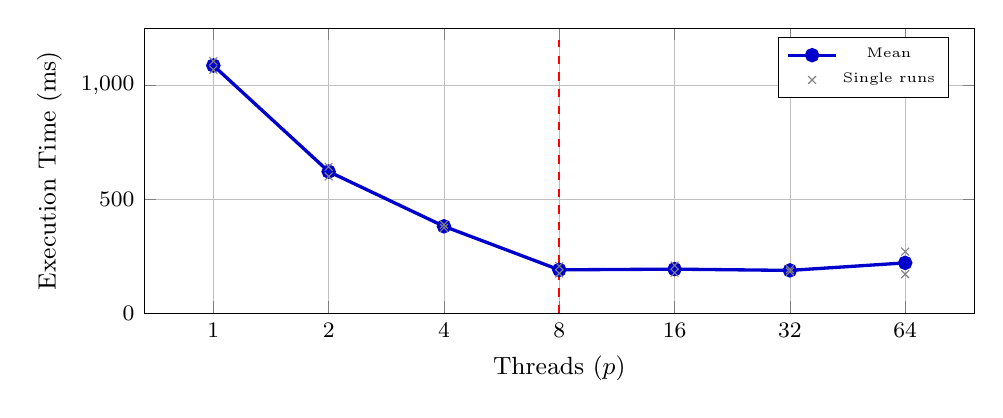
\begin{tikzpicture}
\begin{axis}[
    width=\textwidth, height=5.2cm,
    xlabel={Threads ($p$)}, ylabel={Execution Time (ms)},
    symbolic x coords={1, 2, 4, 8, 16, 32, 64}, xtick=data,
    ymin=0, ymax=1250,
    legend pos=north east, legend style={font=\tiny},
    grid=both,
    grid style={line width=.1pt, draw=gray!25},
    major grid style={line width=.2pt,draw=gray!50},
    tick label style={font=\footnotesize},
    label style={font=\small},
]
    \addplot[color=blue!80!black, mark=*, line width=1.2pt] coordinates {
        (1, 1086.5) (2, 621) (4, 381) (8, 190) (16, 193) (32, 187.5) (64, 220.5)
    };
    \addlegendentry{Mean}
    \addplot[only marks, color=gray, mark=x] coordinates {
        (1, 1068) (2, 600) (4, 388) (8, 206) (16, 177) (32, 193) (64, 171)
        (1, 1105) (2, 642) (4, 374) (8, 174) (16, 209) (32, 182) (64, 270)
    };
    \addlegendentry{Single runs}
    \draw[dashed, red, line width=0.8pt] (axis cs:8,0) -- (axis cs:8,1200);
\end{axis}
\end{tikzpicture}
\caption{Wall-Clock Execution Time}
\end{subfigure}
\hfill
\begin{subfigure}[b]{0.48\textwidth}
\centering
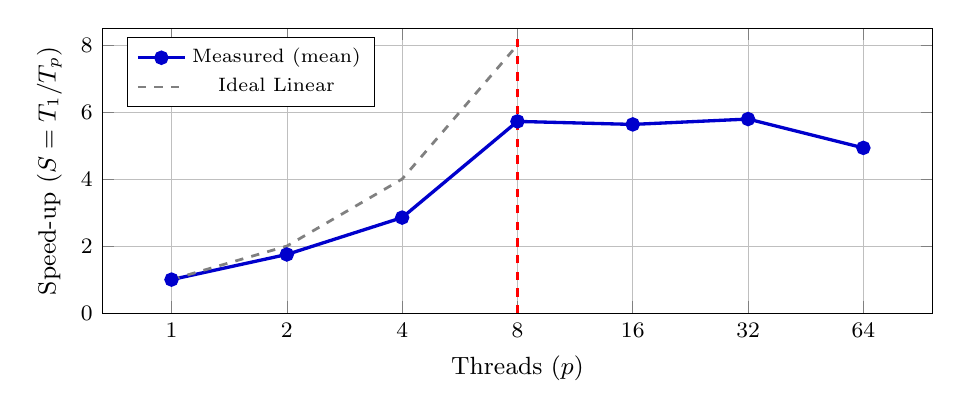
\begin{tikzpicture}
\begin{axis}[
    width=\textwidth, height=5.2cm,
    xlabel={Threads ($p$)}, ylabel={Speed-up ($S = T_1 / T_p$)},
    symbolic x coords={1, 2, 4, 8, 16, 32, 64}, xtick=data,
    ymin=0, ymax=8.5,
    legend pos=north west, legend style={font=\scriptsize},
    grid=both,
    grid style={line width=.1pt, draw=gray!25},
    major grid style={line width=.2pt,draw=gray!50},
    tick label style={font=\footnotesize},
    label style={font=\small},
]
    \addplot[color=blue!80!black, mark=*, line width=1.2pt] coordinates {
        (1, 1.00) (2, 1.75) (4, 2.85) (8, 5.72) (16, 5.63) (32, 5.79) (64, 4.93)
    };
    \addlegendentry{Measured (mean)}
    \addplot[color=gray, dashed, line width=1pt] coordinates {
        (1, 1) (2, 2) (4, 4) (8, 8)
    };
    \addlegendentry{Ideal Linear}
    \draw[dashed, red, line width=0.8pt] (axis cs:8,0) -- (axis cs:8,8.2);
\end{axis}
\end{tikzpicture}
\caption{Parallel Speed-up}
\end{subfigure}
\caption{Task 1a: Wall-Clock Execution Time and Parallel Speed-up vs. Number of Threads ($p$); the red line marks the 8 cores}
\label{fig:task1a}
\end{figure}

\begin{figure}[H]
\centering
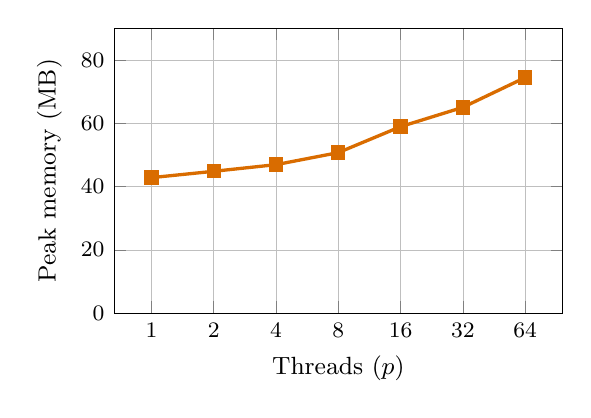
\begin{tikzpicture}
\begin{axis}[
    width=0.6\textwidth, height=5.2cm,
    xlabel={Threads ($p$)}, ylabel={Peak memory (MB)},
    symbolic x coords={1, 2, 4, 8, 16, 32, 64}, xtick=data,
    ymin=0, ymax=90,
    grid=both,
    grid style={line width=.1pt, draw=gray!25},
    major grid style={line width=.2pt,draw=gray!50},
    tick label style={font=\footnotesize},
    label style={font=\small},
]
    \addplot[color=orange!85!black, mark=square*, line width=1.2pt] coordinates {
        (1, 42.8) (2, 44.8) (4, 46.9) (8, 50.7) (16, 58.9) (32, 65.0) (64, 74.4)
    };
\end{axis}
\end{tikzpicture}
\caption{Task 1a: Peak memory vs. number of threads}
\label{fig:task1a_mem}
\end{figure}

\subsection{Task 1b Benchmark Results}
Table~\ref{tab:task1b} compares timing and counter integrity across the three synchronization approaches executed with 8 threads (one per logical processor).

\begin{table}[H]
\centering
\caption{Task 1b: Synchronization Strategy Performance ($p = 8$ threads)}
\label{tab:task1b}
\vspace{2mm}
\small
\setlength{\tabcolsep}{4pt}
\begin{tabular}{lcccc}
\toprule
\textbf{Strategy} & \textbf{Run} & \textbf{Time (ms)} & \textbf{Total Count} & \textbf{Integrity Result} \\
\midrule
Unsynchronized (Race) & Run 1 & 54 & $9\,706\,011$ & Corrupted ($-80.6\%$) \\
Unsynchronized (Race) & Run 2 & 53 & $9\,996\,981$ & Corrupted ($-80.0\%$) \\
Unsynchronized (Race) & Run 3 & 46 & $8\,619\,866$ & Corrupted ($-82.8\%$) \\
Lock-Protected (\texttt{lock}) & -- & 951 & $50\,000\,000$ & Correct (slow) \\
Thread-Local Accumulators & -- & \textbf{37} & $50\,000\,000$ & Correct (fastest) \\
\bottomrule
\end{tabular}
\end{table}

The three unsynchronized runs give three different totals, which is the signature of a race condition: the result depends on the timing of the interleaving, not on the input. Their average time is $51$~ms. In the ``Integrity'' column the percentage is the share of the $50\,000\,000$ updates that was lost. Version 3 is about $26\times$ faster than the lock.

\subsection{Task 1c Benchmark Results}
Table~\ref{tab:task1c} displays the pipeline throughput with 1 producer reader and varying consumer worker counts. As in Task 1a, every configuration was run twice; the speed-up is computed from the mean and the peak memory comes from run 2. All runs produced the checksum $50\,000\,000$.

\begin{table}[H]
\centering
\caption{Task 1c: Producer-Consumer Throughput and Memory vs. Consumer Workers}
\label{tab:task1c}
\vspace{2mm}
\small
\setlength{\tabcolsep}{5pt}
\resizebox{\textwidth}{!}{%
\begin{tabular}{cccccc}
\toprule
\textbf{Workers ($w$)} & \textbf{Run 1 (ms)} & \textbf{Run 2 (ms)} & \textbf{Mean (ms)} & \textbf{Speed-up vs. 1W} & \textbf{Peak RAM (MB)} \\
\midrule
1  & 1714 & 1612 & 1663.0 & $1.00\times$ & 123.1 \\
2  & 1517 & 1520 & 1518.5 & $1.10\times$ & 55.9  \\
4  & 1723 & 1714 & 1718.5 & $0.97\times$ & 70.0  \\
8  & 1990 & 1893 & 1941.5 & $0.86\times$ & 67.8  \\
16 & 2297 & 2175 & 2236.0 & $0.74\times$ & 70.1  \\
32 & 3238 & 3256 & 3247.0 & $0.51\times$ & 94.8  \\
64 & 4028 & 4187 & 4107.5 & $0.40\times$ & 129.4 \\
\bottomrule
\end{tabular}}
\end{table}

\begin{figure}[H]
\centering
\begin{subfigure}[b]{0.48\textwidth}
\centering
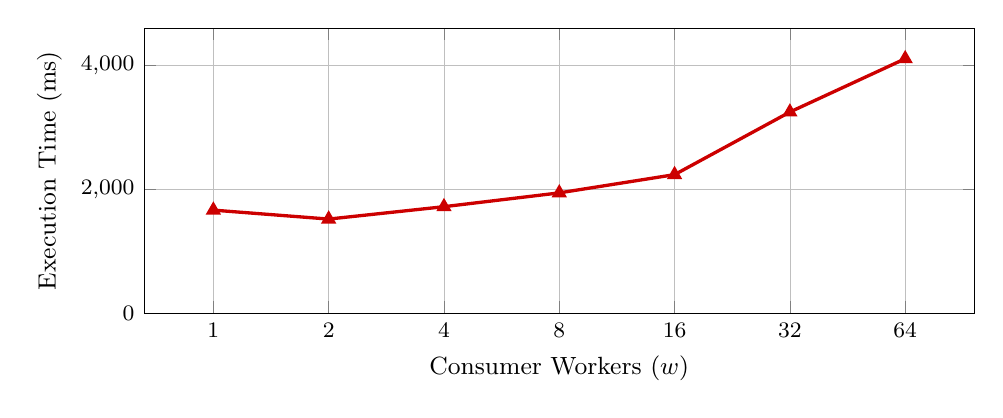
\begin{tikzpicture}
\begin{axis}[
    width=\textwidth, height=5.2cm,
    xlabel={Consumer Workers ($w$)}, ylabel={Execution Time (ms)},
    symbolic x coords={1, 2, 4, 8, 16, 32, 64}, xtick=data,
    ymin=0, ymax=4600,
    grid=both,
    grid style={line width=.1pt, draw=gray!25},
    major grid style={line width=.2pt,draw=gray!50},
    tick label style={font=\footnotesize},
    label style={font=\small},
]
    \addplot[color=red!80!black, mark=triangle*, line width=1.2pt] coordinates {
        (1, 1663) (2, 1518.5) (4, 1718.5) (8, 1941.5) (16, 2236) (32, 3247) (64, 4107.5)
    };
\end{axis}
\end{tikzpicture}
\caption{Wall-Clock Execution Time (mean)}
\end{subfigure}
\hfill
\begin{subfigure}[b]{0.48\textwidth}
\centering
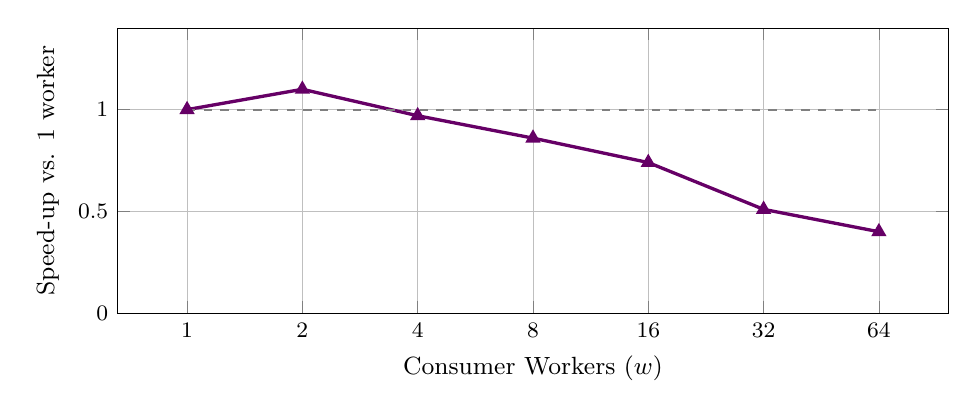
\begin{tikzpicture}
\begin{axis}[
    width=\textwidth, height=5.2cm,
    xlabel={Consumer Workers ($w$)}, ylabel={Speed-up vs. 1 worker},
    symbolic x coords={1, 2, 4, 8, 16, 32, 64}, xtick=data,
    ymin=0, ymax=1.4,
    grid=both,
    grid style={line width=.1pt, draw=gray!25},
    major grid style={line width=.2pt,draw=gray!50},
    tick label style={font=\footnotesize},
    label style={font=\small},
]
    \addplot[color=violet!80!black, mark=triangle*, line width=1.2pt] coordinates {
        (1, 1.00) (2, 1.10) (4, 0.97) (8, 0.86) (16, 0.74) (32, 0.51) (64, 0.40)
    };
    \draw[dashed, gray, line width=0.8pt] (axis cs:1,1) -- (axis cs:64,1);
\end{axis}
\end{tikzpicture}
\caption{Speed-up Relative to One Worker}
\end{subfigure}
\caption{Task 1c: Producer-Consumer Pipeline vs. Number of Consumer Workers}
\label{fig:task1c}
\end{figure}

\begin{figure}[H]
\centering
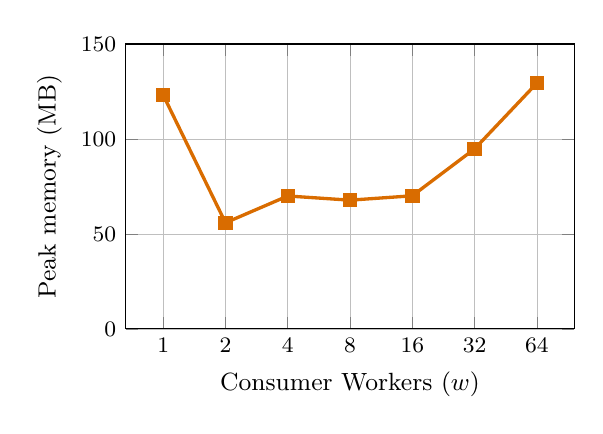
\begin{tikzpicture}
\begin{axis}[
    width=0.6\textwidth, height=5.2cm,
    xlabel={Consumer Workers ($w$)}, ylabel={Peak memory (MB)},
    symbolic x coords={1, 2, 4, 8, 16, 32, 64}, xtick=data,
    ymin=0, ymax=150,
    grid=both,
    grid style={line width=.1pt, draw=gray!25},
    major grid style={line width=.2pt,draw=gray!50},
    tick label style={font=\footnotesize},
    label style={font=\small},
]
    \addplot[color=orange!85!black, mark=square*, line width=1.2pt] coordinates {
        (1, 123.1) (2, 55.9) (4, 70.0) (8, 67.8) (16, 70.1) (32, 94.8) (64, 129.4)
    };
\end{axis}
\end{tikzpicture}
\caption{Task 1c: Peak memory vs. number of consumer workers}
\label{fig:task1c_mem}
\end{figure}

\subsection{Task 2 Benchmark Results}
Table~\ref{tab:task2} presents the multi-file ingestion performance on the USB drive, one run per thread count. Task 2 was run on the same MacBook Air as Tasks 1a--1c, so the reference for the comparison is Task 1a with one thread: $1086.5$~ms (mean of the two runs of Table~\ref{tab:task1a}). The drive is a Kingston DataTraveler 3.0, which supports USB 3.0, but through the USB-C adapter used here it was enumerated by macOS at \emph{Full Speed} (12~Mb/s, \texttt{Device Speed} = 1), whose practical limit is about $1$~MB/s. This is the speed measured in all runs below.

\begin{table}[H]
\centering
\caption{Task 2: USB Drive Multi-File Processing vs. Thread Count (cold cache)}
\label{tab:task2}
\vspace{2mm}
\footnotesize
\setlength{\tabcolsep}{4pt}
\resizebox{\textwidth}{!}{%
\begin{tabular}{ccccccc}
\toprule
\textbf{Threads} & \textbf{Total (s)} & \textbf{Speed-up} & \textbf{Read, per thread (s)} & \textbf{Parse, per thread (s)} & \textbf{Peak RAM (MB)} & \textbf{Checksum} \\
\midrule
1 & 354.730 & $1.00\times$ & 353.961 & 0.768 & 87.4  & $50\,000\,000$ \\
2 & 320.829 & $1.11\times$ & 280.125 / 320.434 & 0.398 / 0.394 & 218.4 & $50\,000\,000$ \\
4 & 333.283 & $1.06\times$ & 274.347 / 333.094 / 292.774 / 285.304 & 0.188--0.196 & 308.5 & $50\,000\,000$ \\
\bottomrule
\end{tabular}}
\end{table}

\begin{figure}[H]
\centering
\begin{subfigure}[b]{0.48\textwidth}
\centering
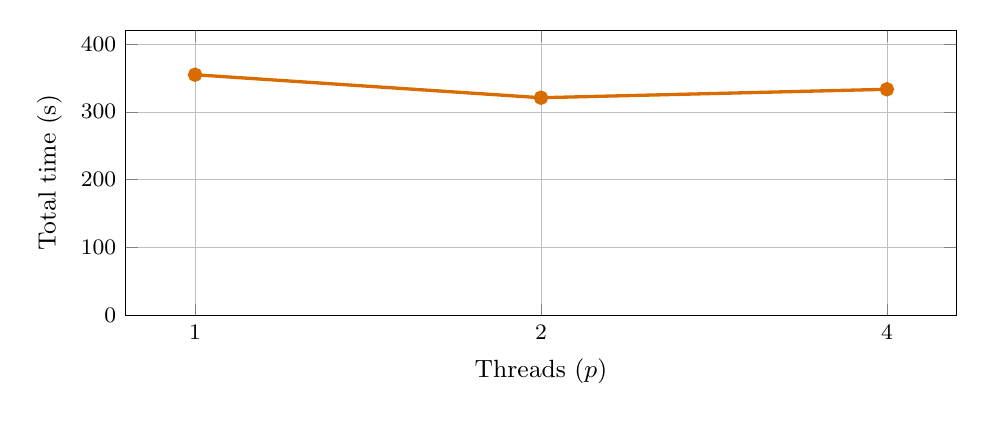
\begin{tikzpicture}
\begin{axis}[
    width=\textwidth, height=5.2cm,
    xlabel={Threads ($p$)}, ylabel={Total time (s)},
    symbolic x coords={1, 2, 4}, xtick=data,
    ymin=0, ymax=420,
    grid=both, grid style={line width=.1pt, draw=gray!25},
    major grid style={line width=.2pt,draw=gray!50},
    tick label style={font=\footnotesize}, label style={font=\small},
]
    \addplot[color=orange!85!black, mark=*, line width=1.2pt] coordinates { (1, 354.73) (2, 320.83) (4, 333.28) };
\end{axis}
\end{tikzpicture}
\caption{Execution time}
\end{subfigure}
\hfill
\begin{subfigure}[b]{0.48\textwidth}
\centering
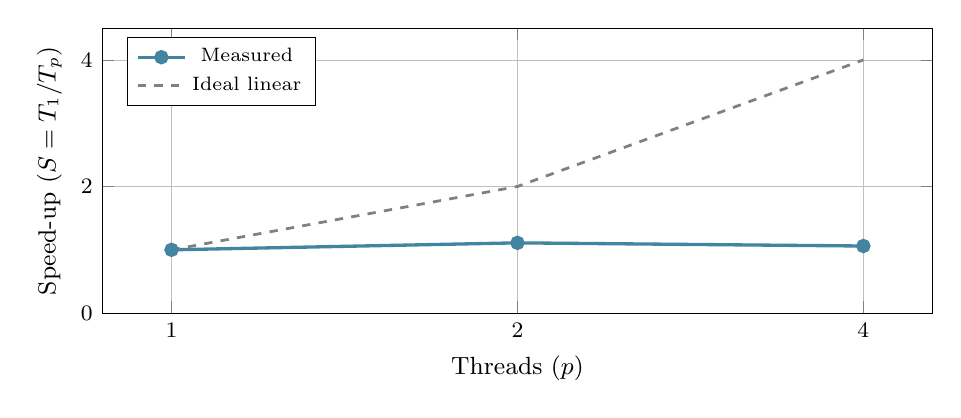
\begin{tikzpicture}
\begin{axis}[
    width=\textwidth, height=5.2cm,
    xlabel={Threads ($p$)}, ylabel={Speed-up ($S = T_1 / T_p$)},
    symbolic x coords={1, 2, 4}, xtick=data,
    ymin=0, ymax=4.5,
    legend pos=north west, legend style={font=\scriptsize},
    grid=both, grid style={line width=.1pt, draw=gray!25},
    major grid style={line width=.2pt,draw=gray!50},
    tick label style={font=\footnotesize}, label style={font=\small},
]
    \addplot[color=cyan!60!black, mark=*, line width=1.2pt] coordinates { (1, 1.00) (2, 1.11) (4, 1.06) };
    \addlegendentry{Measured}
    \addplot[color=gray, dashed, line width=1pt] coordinates { (1, 1) (2, 2) (4, 4) };
    \addlegendentry{Ideal linear}
\end{axis}
\end{tikzpicture}
\caption{Speed-up}
\end{subfigure}
\caption{Task 2: execution time and speed-up on the USB drive}
\label{fig:task2}
\end{figure}

\begin{figure}[H]
\centering
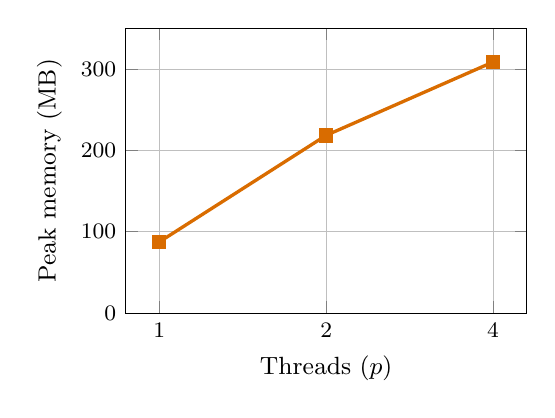
\begin{tikzpicture}
\begin{axis}[
    width=0.55\textwidth, height=5.2cm,
    xlabel={Threads ($p$)}, ylabel={Peak memory (MB)},
    symbolic x coords={1, 2, 4}, xtick=data,
    ymin=0, ymax=350,
    grid=both, grid style={line width=.1pt, draw=gray!25},
    major grid style={line width=.2pt,draw=gray!50},
    tick label style={font=\footnotesize}, label style={font=\small},
]
    \addplot[color=orange!85!black, mark=square*, line width=1.2pt] coordinates { (1, 87.4) (2, 218.4) (4, 308.5) };
\end{axis}
\end{tikzpicture}
\caption{Task 2: peak memory vs. number of threads}
\label{fig:task2_mem}
\end{figure}

\textbf{Measurement protocol.} Before every run the operating system file cache was emptied with \texttt{sudo purge}. The procedure of the laboratory asks for ejecting and re-plugging the drive, but macOS refused to unmount it (the service \texttt{storagekitd} dissented), so \texttt{sudo purge} was used instead for all three runs; this is a deviation from the prescribed procedure. Earlier runs, made without emptying the cache between them, were discarded: they gave inconsistent times ($21.6$, $9.9$ and $48.1$~s for one thread), and in the four-thread case two threads read two 44~MiB files in $0.02$--$0.05$~s, which is only possible from the cache. In the runs of Table~\ref{tab:task2} every thread needed seconds to hundreds of seconds for reading, i.e. the data really came from the drive.

\textbf{Memory.} The peak memory grows with the number of threads ($87.4$, $218.4$ and $308.5$~MB), because every thread holds the whole content of the file it is processing in one byte buffer (about 44~MiB per file) and buffers of files already processed wait for garbage collection.

% =========================================================================
% SECTION 6: TASK QUESTIONS AND CRITICAL ANALYSIS
% =========================================================================
\section{Task Questions and Critical Analysis}

\subsection{Task 1 Questions}

\subsubsection{Question 1: At which number of threads does the speed-up stop growing? Relate it to physical cores and logical processors.}
Speed-up grows up to \textbf{8 threads}: $1.75\times$ at 2 threads, $2.85\times$ at 4 and $5.72\times$ at 8 ($190$~ms, mean of two runs). The M3 has 8 physical cores and 8 logical processors ($P = L = 8$, no SMT), and 8 is exactly where the growth stops: with 16 and 32 threads the speed-up stays at $5.63\times$ and $5.79\times$, within the run-to-run variation, and at 64 threads it falls to $4.93\times$. The speed-up at 8 threads is below the ideal $8\times$ (efficiency $71.5\%$). Probable reasons are that 4 of the 8 cores are slower efficiency cores, that all threads share the same memory bandwidth and the OS file cache while streaming a 352~MB file, and that the serial part (thread creation, file opening, final reduction) does not shrink. The efficiency also drops between 2 and 4 threads ($87.5\%$ to $71.3\%$), before the E-cores are needed, which points to the shared memory/cache system as one of the limits.

\subsubsection{Question 2: Why do 32 and 64 threads not help? Are they slower, and why?}
With 8 logical processors, only 8 threads can run at the same time; the extra threads only wait for a core, so no additional computation can be done per second. With 16 and 32 threads the time ($193$ and $188$~ms) is practically the same as with 8 threads ($190$~ms): each thread has a short, independent job (parsing its own byte range, with no shared state and no locks), so the additional context switches cost little. With 64 threads the mean time rises to $220.5$~ms, about $16\%$ slower than with 8 threads, although the two runs disagree ($171$~ms and $270$~ms): the overhead of creating and scheduling 64 threads, each opening its own file handle and 1~MB buffer, becomes visible and unstable. The efficiency falls from $71.5\%$ at 8 threads to $7.7\%$ at 64 threads: the extra threads consume resources (see Question 3) without delivering speed-up.

\subsubsection{Question 3: Does the peak memory depend on the number of threads? Why?}
Yes. In Task 1a the peak memory grows from $42.8$~MB with 1 thread to $74.4$~MB with 64 threads, an increase of $31.6$~MB, i.e. about $0.5$~MB per additional thread. Every thread reserves an execution stack and, in our implementation, allocates a 1~MB buffer (\texttt{new BufferedStream(fs, 1 << 20)}). The measured growth is half of the nominal $1$~MB per thread because the operating system counts only the pages that have actually been touched. In Task 1c the memory depends much less on the number of workers for $2$--$16$ workers ($55.9$--$70.1$~MB), because the bounded queue (at most 100 batches of $10\,000$ lines) limits the data held in memory; it grows again for 32 and 64 workers ($94.8$ and $129.4$~MB) because of the per-thread stacks and the larger amount of work for the garbage collector. The highest value at one worker ($123.1$~MB) is probably due to the single worker being slower than the reader, so that the queue is filled to its limit of 100 batches, while with several workers the queue stays almost empty. Peak memory was measured once per configuration (run 2), so differences of a few MB should not be over-interpreted.

\subsubsection{Question 4: Rank the three versions of Task 1b by time. Which of them are correct? Explain each result.}
The ranking by time is:
\begin{center}
\textbf{Thread-Local Accumulators (37~ms) $<$ Unsynchronized Shared Counters (51~ms avg.) $\ll$ Lock-Protected Counters (951~ms)}
\end{center}
Only versions 2 and 3 are correct.
\begin{itemize}
    \item \textbf{Thread-Local Accumulators (correct, 37~ms)}: Each thread updates its own local variables, held in registers or its own cache lines, so no cache-coherence traffic occurs between cores until the final sum of 8 values.
    \item \textbf{Unsynchronized Shared Counters (incorrect, 46--54~ms)}: There is no waiting and no kernel involvement, so it is much faster than the lock, but the result is wrong: the three runs returned totals between $8.6$ and $10.0$~million instead of $50$~million, i.e. about $81\%$ of the updates were lost. It is also slower than version 3 (about $38\%$ on average) because all cores keep invalidating the same cache line.
    \item \textbf{Lock-Protected Counters (correct, 951~ms)}: The lock makes every increment a serialized critical section. The 8 threads compete for the lock and for the cache line that holds the counters, so execution is effectively sequential and burdened by lock acquisition and release; it is about $26\times$ slower than version 3 and $19\times$ slower than the unsynchronized version.
\end{itemize}

\subsubsection{Question 5: Compare Task 1c with Task 1a. Which one is faster, and why? At which number of workers does Task 1c stop getting faster?}
Task 1a is much faster: its best mean time is about $190$~ms (8 threads), while the best mean time of Task 1c is $1518.5$~ms (2 workers), i.e. about $8\times$ slower. Even with a single thread/worker, Task 1c ($1663$~ms) is about $1.5\times$ slower than Task 1a ($1086.5$~ms). In Task 1a every thread reads and parses its own part of the file independently, with no coordination. In Task 1c a single reader thread must read the whole file line by line, allocate a string for each of the $50\,000\,000$ lines and pass the batches through a shared queue, so the reader is the bottleneck and the parallel workers mostly wait for it. Task 1c stops getting faster at \textbf{2 workers} ($1.10\times$ speed-up); with 4 workers the time is already slightly worse than with 1 worker ($0.97\times$), and with more workers it gets steadily worse ($0.40\times$ at 64 workers), probably because of contention on the shared queue, context switching among the waiting workers and more garbage-collection work.

\subsubsection{Question 6: What would happen with batches of a single line? And with a queue that has no size limit?}
\begin{itemize}
    \item \textbf{Single-Line Batches}: Throughput would drop sharply. For every one of the $50\,000\,000$ numbers the queue lock would be taken, an array object allocated and waiting threads signalled, and this overhead would be much larger than the cost of parsing and counting one number.
    \item \textbf{Unbounded Queue}: The reader (which is faster than the workers when there are few workers) could run ahead and read all $50\,000\,000$ lines into memory as strings. This would need roughly 2~GB of heap, cause heavy garbage-collection pressure and, on a machine with less memory, could end in an \texttt{OutOfMemoryException} or swapping. The bound of 100 batches (about $10^6$ lines) keeps memory constant.
\end{itemize}

\subsection{Task 2 Questions}

\subsubsection{Question 1: Compare the time on one thread with Task 1a on one thread. On the USB drive, is the work CPU-bound or I/O-bound?}
Task 1a with one thread, reading from the internal SSD, takes $1086.5$~ms (mean). Task 2 with one thread on the USB drive takes $354.730$~s, about $326\times$ longer for the same $50\,000\,000$ numbers. Of this time, $353.961$~s ($99.8\%$) is spent reading from the drive and only $0.768$~s parsing and counting, which is shorter than the whole Task 1a run. The effective read throughput is about $369$~MB $/\ 354$~s $\approx 1.0$~MB/s, which matches the practical limit of a Full Speed (12~Mb/s) USB link. On the USB drive the work is therefore \textbf{I/O-bound}: the CPU is idle for more than $99\%$ of the time waiting for the drive. On the internal SSD (Task 1a) the data arrive much faster than they can be parsed, and adding cores gave a $5$--$6\times$ speed-up, so that work is \textbf{CPU-bound}.

\subsubsection{Question 2: On the USB drive, do more threads help? Why not, when lecture 1 showed that I/O-bound work benefits from concurrency?}
No. The time is $354.7$~s with 1 thread, $320.8$~s with 2 threads ($1.11\times$) and $333.3$~s with 4 threads ($1.06\times$): the speed-up is far from the ideal $2\times$ and $4\times$, and the four-thread run is even slower than the two-thread run. The small differences ($6$--$11\%$) are of the order of the variation of such a slow link and cannot be attributed to the threads; overlapping the parsing of the threads could save at most $0.77$~s of the $354$~s. Lecture~1 showed that concurrency helps I/O-bound work when the time is spent \emph{waiting} for many independent sources, for example many network servers, whose waiting times overlap. Here all threads wait for the \emph{same} device behind one USB link: the bandwidth of about $1$~MB/s is a shared resource, so a second or fourth reader receives only a part of it and the total time is determined by the number of bytes divided by this bandwidth ($369$~MB $/\ 1.04$~MB/s $\approx 354$~s), independently of how many threads request them. In the per-thread data the threads indeed read at the same time for about $275$--$333$~s each, which is the whole run, while the work they could do in parallel (parsing, $0.19$--$0.77$~s) is negligible.

% =========================================================================
% SECTION 7: ANSWERS TO CONTROL QUESTIONS
% =========================================================================
\section{Answers to Control Questions}

\subsection{1. Difference between a physical core and a logical processor; how did it show in your charts?}
A physical core is an independent processing unit on the silicon die containing its own execution units, instruction decoders, and L1 caches. A logical processor is what the operating system schedules threads on. With Simultaneous Multithreading (Intel Hyper-Threading), one physical core presents two logical processors that share its execution units.

On our host (Apple M3) there are 8 physical cores (4 performance + 4 efficiency) and 8 logical processors, because Apple cores do not use SMT. In our charts:
\begin{itemize}
    \item From 1 to 4 threads the mean time decreases from $1086.5$ to $381$~ms ($2.85\times$).
    \item From 4 to 8 threads, when all 8 cores (including the slower E-cores) are in use, the time falls to $190$~ms ($5.72\times$).
    \item Beyond 8 threads (16, 32, 64) the speed-up stays at about $5.6$--$5.8\times$ and drops to $4.9\times$ at 64 threads: the number of threads exceeds the number of logical processors and no more work can run simultaneously. The change of the curve at $p = 8$ marks the equality of physical cores and logical processors on this machine.
\end{itemize}

\subsection{2. How did you make sure that no line was counted twice or skipped at the boundary between two parts of the file?}
\begin{enumerate}
    \item The file of size $S$ is divided into $N$ byte ranges $[B_i, B_{i+1})$ with $B_i = \lfloor iS/N \rfloor$.
    \item A thread $i > 0$ starts at byte $B_i - 1$ and reads forward until the first \texttt{'\textbackslash n'}, discarding that (possibly partial) line. If the byte $B_i - 1$ is itself a newline, the thread begins exactly at $B_i$.
    \item Thread $i$ then parses complete lines for as long as the line starts before $B_{i+1}$; the last line may therefore extend past $B_{i+1}$.
    \item Thread $i+1$ discards everything up to the first newline after $B_{i+1} - 1$, which is exactly the end of that last line. Every line is therefore counted by exactly one thread. This is confirmed by the totals: all runs sum to $50\,000\,000$ with identical counts of negative, positive and zero values.
\end{enumerate}

\subsection{3. Explain step by step how unsynchronised shared counters lose updates.}
At the machine level, an increment operation \texttt{counter++} consists of three discrete operations:
\begin{center}
1. Load: $R \leftarrow [\text{addr}] \quad \longrightarrow \quad$ 2. Add: $R \leftarrow R + 1 \quad \longrightarrow \quad$ 3. Store: $[\text{addr}] \leftarrow R$
\end{center}
Consider two threads ($T_A$ and $T_B$) executing concurrently when counter has value 100:
\begin{enumerate}
    \item $T_A$ reads counter ($R_A = 100$).
    \item $T_B$ reads counter before $T_A$ writes ($R_B = 100$).
    \item $T_A$ increments its register ($R_A = 101$).
    \item $T_B$ increments its register ($R_B = 101$).
    \item $T_A$ writes back $101$.
    \item $T_B$ writes back $101$.
\end{enumerate}
Two increments occurred, but the value increased only by 1: one update was lost. With 8 threads incrementing the same three counters $50\,000\,000$ times, this happened so often that only about $19\%$ of the increments survived in our runs (totals of $8.6$--$10.0$~million).

\subsection{4. Why are per-thread counters faster than shared counters protected by a lock?}
\begin{itemize}
    \item \textbf{Cache-coherence traffic}: When several cores modify one shared counter, its cache line must move between the cores' caches on every write, invalidating the copies in the other cores and forcing them to wait.
    \item \textbf{Serialization}: A lock allows only one thread at a time in the critical section, so 8 threads behave like one thread plus the cost of acquiring and releasing the lock for each of the $50\,000\,000$ increments (951~ms in our measurement).
    \item \textbf{Independence}: Per-thread counters live in registers or in separate memory, so each core works on its own L1 cache with no communication; the 8 partial results are added only once at the end (37~ms).
\end{itemize}

\subsection{5. What does ``I/O-bound'' mean for a USB drive, and for a server waiting on the network? Why does concurrency help in only one of the two cases?}
An operation is I/O-bound when its speed is limited by an input/output subsystem rather than by the CPU.
\begin{itemize}
    \item \textbf{USB drive}: The limit is the bandwidth of one device and one bus. The CPU is mostly waiting for the data, but more threads cannot make the drive deliver more bytes per second, so concurrency does not help.
    \item \textbf{Network server}: The time is spent waiting for many independent remote parties (clients, databases, other servers), each of them with its own latency. While one connection waits, the CPU can handle another, so concurrency (or asynchronous I/O) overlaps the waiting times and increases throughput.
\end{itemize}

\subsection{6. What is the difference between dividing the work into equal parts in advance and taking it from a queue? When is each one better?}
\begin{itemize}
    \item \textbf{Static partitioning (dividing in advance)}: The data is divided into $N$ chunks before execution, one per worker.
    \begin{itemize}
        \item \textit{Advantages}: no coordination during execution, no queue overhead, good cache locality (Task 1a: about $190$~ms).
        \item \textit{When better}: when all items cost about the same and the amount of work is known in advance.
    \end{itemize}
    \item \textbf{Dynamic queue}: Workers take the next available batch from a shared queue.
    \begin{itemize}
        \item \textit{Advantages}: automatic load balancing, works for streaming data whose size is not known in advance, bounded memory with a bounded queue.
        \item \textit{When better}: when the cost per item varies unpredictably, or when the producer cannot be split in advance. For this lab's uniform workload the queue was slower (Task 1c: $1518.5$~ms at best) because the single reader is a bottleneck.
    \end{itemize}
\end{itemize}

% =========================================================================
% SECTION 8: CONCLUSIONS
% =========================================================================
\section{Conclusions}

Using a workload of $50\,000\,000$ integers on an Apple M3 (8 cores, no SMT) the following conclusions were obtained:
\begin{enumerate}
    \item \textbf{Hardware saturation limits}: Speed-up grows up to the 8 cores of the processor ($5.72\times$ at 8 threads, $1086.5 \to 190$~ms) and does not grow afterwards ($5.6$--$5.8\times$ for 16 and 32 threads, $4.9\times$ for 64). Task 1a is therefore \textbf{CPU-bound} on the internal SSD: the parsing speed, not the disk, limits the time. Peak memory grows with the number of threads ($42.8 \to 74.4$~MB).
    \item \textbf{Cost of synchronization}: Unsynchronized shared counters are fast but wrong ($\approx 81\%$ of updates lost, a different result in each run). The lock makes the result correct but $\approx 26\times$ slower than per-thread counters (951~ms vs. 37~ms), which are both correct and the fastest.
    \item \textbf{Producer-consumer}: With one reader, adding workers does not help: the best time ($1518.5$~ms at 2 workers) is about $8\times$ slower than static partitioning, and more than 2 workers make it worse ($4107.5$~ms at 64).
    \item \textbf{Slow storage}: On the USB drive, which worked at Full Speed (12~Mb/s) through the adapter, one thread needed $354.7$~s, of which $99.8\%$ was reading (about $1.0$~MB/s), versus $1.09$~s on the internal SSD: the work is I/O-bound on the drive and CPU-bound on the SSD. More threads did not help ($1.11\times$ with 2 and $1.06\times$ with 4 threads), because all threads share the same slow device and bus.
\end{enumerate}

% =========================================================================
% SECTION 9: SOURCE CODE AND BUILD INSTRUCTIONS
% =========================================================================
\section{Source Code and Build Instructions}

The source code is available in the repository:
\begin{center}
\url{https://github.com/don09dandidi/PR}
\end{center}

\subsection{Build and Execution Commands}
Requirements: .NET 10 SDK. Commands are run from the \texttt{lab1} directory (macOS or Linux shell syntax; on Windows use the drive letter instead of the \texttt{/Volumes} path).

\begin{lstlisting}[language=bash]
cd lab1

# Build in Release configuration
dotnet build -c Release

# 1. Generate numbers.txt (50 million integers) and split it into 8 files
dotnet run -c Release -- gen

# 2. Task 1a, one process per configuration
for t in 1 2 4 8 16 32 64; do dotnet run -c Release -- 1a $t; done

# 3. Task 1b (version 1 runs three times)
dotnet run -c Release -- 1b

# 4. Task 1c, one process per configuration
for t in 1 2 4 8 16 32 64; do dotnet run -c Release -- 1c $t; done

# 5. Task 2: copy numbers_*.txt to the USB drive, then empty the
#    file cache before every run:
sudo purge
dotnet run -c Release -- 2 /Volumes/Ventoy 1
sudo purge
dotnet run -c Release -- 2 /Volumes/Ventoy 2
sudo purge
dotnet run -c Release -- 2 /Volumes/Ventoy 4
# (Windows: dotnet run -c Release -- 2 E:\ 1)
\end{lstlisting}

\end{document}